\chapter{Dark Energy and Modified Gravity}

\todo{Heyrovsky D.:

\textit{
the work could have included the observationally most relevant result: the cosmological evolution of the equation of state w(a) predicted by the different modified theories; weak lensing can be analyzed for rich galaxy clusters rather than for single galaxies.}
}

In this chapter we briefly introduce how we can modify Einstein`s general relativity and main ideas behind adding new degrees of freedom to the Einstein equations. We describe one particular model of modified gravity in more detail -- the $f(R)$ theory and chameleon gravity.

% \subsection{Modofied gravity}
\todo{alternatives to the cosmological constant}
Other reasons for studying the modifications of gravity may include the following TODO citation. Modified gravity:
\begin{itemize}
	\item can provide natural unification of the early-time inflation and late-time acceleration TODO CITE
	\item can serve as the basis for unified explanation of dark energy and dark matter TODO CITE
	\item be is expected to be useful in high energy physics TODO CITE
\end{itemize}

\section{\textit{f(R)}-gravity}
\todo{check all equations}
One of the simplest modified gravity models is the so-called $f(R)$ gravity in which we consider general functions of the Ricci scalar $R$ in the action
\eq{
	\label{eq:S_fr}
	S=\frac{\Mpl^2}{2}\int\dd^4x\dg\left[F(R)\right]+S_m[\psi_m;g_\uv]\,,
}
where $F(R)=R+f(R)$ and $S_m$ is the matter action with matter fields $\psi_m$ which are minimally coupled to gravity, i.e. they interact with gravity only through the determinant of the metric $\dg$ and the canonical kinetic term $-\frac12g^\uv\partial_\mu\phi\partial_\nu\phi$. The matter fields $\psi_m$ obey standard conservation equations and therefore the metric $g_\uv$ corresponds to the physical frame -- the Jordan frame.

Variation with respect to the metric $g^\uv$ gives us equation of motion
\eq{
	\label{eq:fR}
	F\R R_\uv-\frac{1}{2}f g_\uv+g_\uv\Box F\R-\nabla_\mu\nabla_\nu F\R=\frac{1}{\Mpl^2}T_\uv\,.
}
For $f(R)=-2\Lambda$ the standard Einstein gravity is reconstructed. Taking the trace of \eqref{eq:fR} we get
\eq{
	\label{eq:fR_tr}
	3\Box F\R+F\R R-2F=\frac{1}{\Mpl^2}T\,.
}
We see that there is a propagating scalar degree of freedom, so-called \textit{scalaron} $F\R$ with mass $m^2=F\R/(3F\RR)$, which corresponds to the scalar field conformally coupled to matter in the Einstein frame.

To get the inflation we need a solution that approaches the de Sitter solution characterized by vacuum space with with a constant positive curvature. Thus $\Box F\R=0$ and \eqref{eq:fR_tr} becomes
\eq{
	F\R R-2f=0.
}
For example the model $f(R)=\alpha R^2$ gives rise to an asymptotically exact de Sitter solution and can be responsible for the inflation in the early Universe. The inflation ends when the quadratic term becomes smaller than the linear term. As at the present epoch is the curvature very small this model is not suitable to realize the present cosmic acceleration. Models like $f(R)=-\alpha/R^n$ with $\alpha>0,\ n>0$ could in principle give rise to the present acceleration. However, these models do not satisfy local gravity constraints because of the instability associated with negative values of $f\RR$. Moreover, the standard matter epoch is not present because of a large coupling between the Ricci scalar and the non-relativistic matter.

There are four conditions for the viability of \fR\ models \parencite{Amendola_2007}
\todo{check literature}
\begin{itemize}
	\item $F\R>0\ (R>R_0)$, where $R_0$ is the Ricci scalar at the present epoch,\\
	-- required to avoid anti-gravity \parencite{2010deto.book.....A}\\
	\item $F\RR>0\ (R>R_0)$,\\
	-- required for consistency with local gravity tests \parencite{2005gr.qc.....5136O}, for the presence of the matter-dominated epoch \parencite{2007PhRvL..98m1302A} and for the stability of cosmological perturbations \parencite{2007PhRvD..75d4004S}\\
	\item $f(R)\rightarrow -2\Lambda\ (R\gg R_0)$,\\
	-- required for consistency with local gravity tests \parencite{2008PhRvD..77b3507T} and for the presence of the matter-dominated epoch \parencite{Amendola_2007}\\
	\item $0<\frac{RF\RR}{F\R}<1\ (F\R R-2f=0)$.\\
	-- required for the stability of the late-time de Sitter solution \parencite{1988PhLB..202..198M}
\end{itemize}
Some examples of \fR\ models that satisfy these conditions:
\eq{
	f(R)&=-\mu R_c(R/R_c)^p	&\mbox{for\ }&0<p<1;\ \mu,R_c>0\,,\\
	f(R)&=-\mu R_c\frac{(R/R_c)^{2n}}{(R/R_c)^{2n}+1} 	&\mbox{for\ }&n,\mu,R_c>0\,,\\
	f(R)&=-\mu R_c\left[1-(1+R^2/R^2_c)^{-n}\right] 	&\mbox{for\ }&n,\mu,R_c>0\,,\\
	f(R)&=-\mu R_c\tanh(R/R_c)	&\mbox{for\ }&\mu,R_c>0\,.
}
One of the main prediction of \fR\ gravity is different structure formation history than in \LCDM. For the large-scale structure formation on subhorizon scales \mbox{$k\gg H$} in quasi-static approximation one gets the modified equation for matter density perturbation \parencite{2011RSPTA.369.4947B}
\eq{
	\ddot{\delta}_m+2H\dot{\delta}_m-4\pi G\eff \rho_m\delta_m\approx0\,,
}
where the effective gravitational constant is defined by
\eq{
	G\eff \equiv\frac{G}{1+f\R}\frac{4k^2+3a^2m^2}{3k^2+3a^2m^2}\,.
}
On scales much larger than the scalaron Compton wavelength $m\mins$, gravity is unmodified aside from the overall reduction factor $f\R$. However, on smaller scales the gravitational coupling increases by the factor $4/3$. As the scalaron mass $m$ and the factor $f\R$ depend on curvature (local density), the chameleon mechanism discussed earlier can prevent the detection of this effect in the Solar System.

%%%%%%%%%%%%%%%%%%%%%%%%%%%%%%
% Jordan vs. Einstein Frame
%%%%%%%%%%%%%%%%%%%%%%%%%%%%%%
\subsection{Jordan vs. Einstein Frame}
\todo{check and fix equations / references}
The action \eqref{eq:S_fr} is described in the so-called Jordan frame, where the matter fields are minimally coupled to the metric and follow geodesics. We can also describe this in the so-called Einstein frame, where ``standard'' gravity is restored. Using the conformal transformations% we can rewrite the action \eqref{eq:S_fr}
\eq{
\label{eins_trans}
\begin{split}
\tilde{g}_\uv &\equiv\varphi g_\uv \\
\left(\frac{\dd \phi}{\dd \varphi}\right)^2 &\equiv\frac{\Mpl^2}{2}\frac{3+2\omega}{\varphi^2} \\
A(\phi) &\equiv\varphi^{-1/2} \\
V(\phi) &\equiv\Mpl^2\frac{U(\varphi)}{\varphi^2}
\end{split}
}
which leads to
\eq{
\label{eq:S_ein_fr}
S=\int\dd^4x\dgt\left[\frac{\Mpl^2}{2}\tilde{R} - \frac12(\partial\phi)^2-V(\phi)\right]+S_m[\psi_m;A^2(\phi)\tilde{g}_\uv],
}
where tildes denote quantities in the Einstein frame. This action looks like the Einstein-Hilbert action with minimally coupled scalar but now the matter fields are also coupled with the scalar field via the factor $A(\phi)$ . %Also from the second row of \eqref{eins_trans} can be seen why is the Brans-Dicke parameter restricted to be $\omega>-3/2$.

There is a difference whether one takes action \eqref{eq:S_fr} or \eqref{eq:S_ein_fr} to be the fundamental action defining the modified gravity. In the former one there is only one coupling constant $\beta$, defined by $A(\phi)=\exp(\beta\phi/\Mpl)$, for all matter fields. If one takes the action in the Einstein frame to be the fundamental one the matter action is replaced by $S_m[\psi_m;A^2(\phi)\tilde{g}_\uv]\rightarrow S_i[\psi_i;A_i^2(\phi)\tilde{g}_\uv]$ where one can define the coupling strengths $\beta_i$ to the different matter components to be different. This is very important for tests of modified gravity. For instance, if there is minimal coupling to the baryonic matter -- $\beta_b=0$, Solar System or astrophysical tests do not constraint coupling strength to the cold matter $\beta_c$ whereas the cosmological observation do.

Also other theories than Jordan-Brans-Dicke theory, e.g. Kaluza-Klein theories and higher derivative theories of gravity, can be formulated in two different ways \parencite{Faraoni:1998qx}.

\todo{rewrite, remove questions}
What does it mean that two frames are conformally related? Are these frames equivalent? And how is this equivality defined? It has been shown in \textcite{Magnano:1993bd} that these two frames are \textit{mathematically} equivalent, i.e. every solution in one frame implies an existence of a solution in the other frame and can be mapped into this frame. But this does not necessary mean that they are \textit{physically} equivalent and quantities defined in the individual frames are those we observe. There has been many debates about the (in)equivalence of these frames \parencite{Postma:2014vaa} and whether which one is the physical \parencite{Faraoni:1999hp}. Many contradictory arguments (sometimes incorrect) of both sides result into confusion and ambiguous viewpoints.

Both frames have some issues with fundamental principles. In the Jordan frame the weak energy condition can be violated and hence states with the negative energy are possible. Moreover, there is no guarantee of stability of ground state. All \textit{classical} fields are believed to satisfy the energy condition but no so in quantum theories. On the other hand in the Einstein frame the weak energy condition is satisfied but due to the non-universal coupling of the matter fields the equivalence principle is violated. However this violation is only weak and can pass the Solar system tests.

\todo{Check literature, update}
So far it has not been definitely decided which frame is the physically correct one or whether they are equivalent and a complete agreement has not been reached in the community on this issue. For more information see e.g. \textcite{Carloni:2009gp,Capozziello:2011et}.
% Magnano, G. and Sokolowski, L.M. (1994), Physical Review D 50, 5039.
% Faraoni, V., Gunzig, E. and Nardone, P. (1998), Fundamentals of Cosmic Physics 20, 121.

%%%%%%%%%%%%%%%%%%%%%%%%%%%%%%
% Screening Mechanisms
%%%%%%%%%%%%%%%%%%%%%%%%%%%%%%
\subsection{Screening Mechanisms}
We know that general relativity with the cosmological constant and assumptions about cold dark matter can describe our universe very well. That means that any modified cosmology must be able to recover \LCDM\ cosmology to a high accuracy. This is not normally an issue. However, since modifications of GR typically involve extra scalar degree of freedom there are interactions with matter that are unavoidable -- no symmetry can prevent all couplings to the standard model. This coupling to matter means that there should be a fifth force. Because we do not see any fifth forces or modifications of gravity in the laboratory or in the Solar System we need to suppress these fifth forces -- we need some sort of a \textit{screening mechanism}.

A nature of the screening mechanisms can be different. Let us start from \eqref{eq:S_ein_fr} with generalized kinetic term $-\frac12 Z(\phi,\partial\phi,...)(\partial\phi)^2$. We can solve the equations of motion for the background in a minimum of a potential $V(\phi)$ and write $\phi=\phi_0+\delta\phi$, where $\phi_0$ is a background solution and $\delta\phi$ is a fluctuation. The Lagrangian density for the fluctuations to the second order (first order vanishes) is
\eq{
\LL\propto-\frac12 Z(\phi_0)(\partial\delta\phi)^2+\frac12 m^2(\phi_0)\delta\phi^2+\frac{\beta(\phi_0)}{M_p}\delta\phi\delta T,
}
where $m^2(\phi)\equiv V_{,\phi\phi}(\phi)$. Now, any of these three terms can serve as a screening term:
\begin{itemize}
	\item  \textit{Large inertia} -- a large $Z$ makes it hard for the scalar to propagate and leads to the kinetic type of the screening, where first or second derivatives being important; e.g. Galileons \parencite{2009PhRvD..79f4036N}, massive gravity \parencite{2012RvMP...84..671H} or Vainshtein mechanism \parencite{2013CQGra..30r4001B};
	\item \textit{Large mass} --  a large $m$ means the scalar propagates only over short distances and leads to the chameleon type of the screening, where in regions of high density, such as on the Earth, the field acquires a large mass -- the Chameleon mechanism \parencite{Waterhouse:2006wv};
	\item \textit{Weak coupling} -- a small $\beta$ in regions of high density makes the interaction with matter fields weaker and leads to symmetron \parencite{2010PhRvL.104w1301H}) or varying dilaton \parencite{Damour:1994zq,2011PhRvD..83j4026B} theories.
\end{itemize}
%%%%%%%%%%%%%%%%%%%%%%%%%%%%
% {Chameleon Gravity
%%%%%%%%%%%%%%%%%%%%%%%%%%%%
\section{Chameleon Gravity}
\label{sec_cham}
If there is a scalar field coupled to a non-relativistic matter with the interaction as strong as gravity, the coupling must be tuned to a small value to satisfy tests of the equivalence principle in Solar System which exclude any fifth forces. However, this fine-tunning can be avoided and the coupling can be of order of unity with the so called \textit{chameleon mechanism}.

The action of a chameleon scalar field $\phi$ is given by the action \eqref{eq:S_ein_fr} in the Einstein frame
\eq{
	\label{cham}
	S=\int\dd^4x\dg\left[\frac{\Mpl^2}{2}R - \frac12(\partial\phi)^2-V(\phi)\right]+S_m[\psi_m^{(i)};g_\uv^{(i)}].
}
It is the same action as for the normal quintessence but now the matter fields are coupled to a metric $g_\uv^{(i)}$, which is related to the Einstein frame metric $g_\uv$ by a conformal transformation
\eq{
	\label{cnf_cpl}
	g_\uv^{(i)}=e^{2\beta_i\phi/\Mpl}g_\uv.
}
Varying the action \eqref{cham} with respect to the field $\phi$ one can obtain the equation of motion
\eq{
	\label{eom:cham}
	\Box\phi=V_{,\phi}-\sum_i\frac{\beta_i}{\Mpl}e^{4\beta_i\phi/\Mpl}g^\uv_{(i)}T^{(i)}_\uv,
}
where
\eq{
	T^{(i)}_\uv\equiv\frac{-2}{\dg}\frac{\delta(\dg\LL_m)}{\delta g^\uv_{(i)}}
}
is the stress-energy tensor for the $i$-th matter component. Note that the stress-energy tensor defined in this way is \textbf{not} conserved in the Einstein frame, but rather in the Jordan frame, i.e.
\eq{
	\tilde{\nabla}_\mu T_{(i)}^\uv=0,
}
where $\tilde{\nabla}_\mu$ is the covariant derivative corresponding to the Jordan frame metric and we are assuming that the individual matter species do not interact with each other. The trace (not a scalar in the Einstein frame) of the $i$-th component is defined as $T^{(i)}\equiv g^\uv_{(i)}T^{(i)}_\uv$. For a perfect isentropic fluid is $T^{(i)}=-(1-3w_i)\tilde{\rho}_i$ with $\tilde{\rho}_i$ the energy density in the Jordan frame. The energy density defined as
\eq{
	\rho_i\equiv\tilde{\rho}_ie^{3(1+w_i)\beta_i\phi/\Mpl},
}
is conserved in the Einstein frame \parencite{Waterhouse:2006wv}.

Equation of motion \eqref{eom:cham} is then
\eq{
	\Box\phi=V_{,\phi}+\sum_i(1-3w_i)\frac{\beta_i}{\Mpl}\rho_i e^{(1-3w_i)\beta_i\phi/\Mpl}.
}
This equation could be read as
\eq{
	\Box\phi=V_{\eff,\phi}\left(\phi\right),
}
where the effective potential $V_{\eff}$ is defined by
\eq{
	V_{\eff}\left(\phi\right)\equiv V(\phi)+\sum_i\rho_i e^{(1-3w_i)\beta_i\phi/\Mpl}.
}
If the couplings $\beta_i$ are the same for each matter component with the same $w$ (we can omit the radiation in the sum) and the overall density is $\rho=\sum_i\rho_i$, then the effective potential reads
\eq{
	V_{\eff}\left(\phi\right)\equiv V(\phi)+\rho e^{(1-3w)\beta\phi/\Mpl}.
}
For the quasi-static and weak $(\beta\phi/\Mpl\ll1)$ field in a weak gravity background (the Minkowski background) with non-relativistic matter, the equation further simplifies as
\eq{
	\label{eq:cham}
	\Delta \phi=\frac{\beta}{\Mpl}\rho+V_{,\phi},
}
which looks like the normal Poisson equation but with an extra non-linear term.
\subsection{Chameleon Force}
The interaction of the chameleon field with matter is described by the conformal coupling \eqref{cnf_cpl}. As the matter fields $\psi_m^{(i)}$ couple to the metric $g_\uv^{(i)}$ instead of $g_\uv$, free test particles follow geodesics of $g_\uv^{(i)}$
\eq{
\frac{\dd^2x^\mu}{\dd\tilde{\tau}^2}+\tilde{\Gamma}^\mu_{\alpha\beta}\dddd{x^\alpha}{\tilde{\tau}}\dddd{x^\beta}{\tilde{\tau}}=0,
}
where $\tilde{\Gamma}^\mu_{\alpha\beta}$ are the Christoffel symbols of the metric $g_\uv^{(i)}$. In the Einstein frame metric this gives \parencite{Waterhouse:2006wv}
\eq{
\frac{\dd^2x^\mu}{\dd\tau^2}+\Gamma^\mu_{\alpha\beta}\dddd{x^\alpha}{\tau}\dddd{x^\beta}{\tau}=-\frac{\beta_i}{\Mpl}\left(2\phi_{,\alpha}\dddd{x^\alpha}{\tau}\dddd{x^\mu}{\tau}+g^{\beta\mu}\phi_{,\beta}\right).
}
Note that the chameleon force violates the weak Equivalence Principle only if there exist two matter species with differing values of $\beta_i$. In the non-relativistic limit, a test particle of mass $m$ of species $i$ in a static chameleon field $\phi$ is moving under a force $\vec{F}_\phi$ given by
\eq{
\label{cham_force}
\frac{\vec{F}_\phi}{m}=-\frac{\beta_i}{\Mpl}\vec{\nabla}\phi
}
\subsection{Chameleon mechanism}
As discussed in \autoref{screen} we need some sort of a screening mechanism to avoid Solar System tests of GR. It means as seen from \eqref{cham_force} that the chameleon potential needs to approach some constant value in dense regions.

Suppose we have a background solution $\phi_\infty$ which minimizes the effective potential with $\rho=\rho_\infty$. For small fluctuations $\phi=\phi_\infty+\delta\phi$ and $\rho=\rho_\infty+\delta\rho$ we can linearized \eqref{eq:cham} to obain
\eq{
\label{eq:cham_lin}
\Delta \delta\phi=\frac{\beta}{\Mpl}\delta\rho+m^2_\infty\delta\phi,
}
where
\eq{
m^2_\infty\equiv V_{,\phi\phi}(\phi_\infty).
}
Except for the screening term, which often could be neglected, the equation \eqref{eq:cham_lin} has the same behavior as the Poisson equation for the Newtonian potential $\Phi_N$. For a spherically symmetric density profile this gives solution
\eq{
\phi=\phi_\infty+2\beta\Mpl\Phi_N\left(r\right)e^{-m_\infty r}.
}
As the objects in the background become more massive (larger and/or denser) the Newtonian potential grows larger (in magnitude) and so the deviation of $\phi$ from background solution $\phi_\infty$. At some point this deviation is no longer small and the potential term in \eqref{eq:cham} cannot be treated perturbatively. It starts canceling the first source term and eventually the field $\phi$ posses a new (constant) value which minimizes the effective potential inside an object.

This is the essence of the chameleon mechanism. Let us derive the mechanism in a more proper and exact way.
\subsection{Chameleon Profile}
\label{cham_prof}
To obtain the cosmic acceleration and chameleon behavior described above we need to choose a chameleon potential $V(\phi)$ with the right properties. As in the case of the quintessence field we need the slow-roll mechanism to provide the acceleration and therefore we need the potential where the field rolls down in a potential slope. To have a screening mechanism in \eqref{eq:cham} we need $V_{,\phi}<0$ and so field rolls down in the positive direction. And finally to have a screening behavior of the field as in  the case of the Yukawa potential we need a real mass of the field, i.e. $V_{,\phi\phi}>0$.

These properties of the potential are commonly referred to as the potential of the \textit{runaway} form:
\begin{enumerate}
	\item $\lim_{\phi \to 0}V\left(\phi\right)=\infty$;
	\item $V\left(\phi\right)$ is $C^\infty$, bounded below;
	\item $V_{,\phi}<0$ and increasing;
	\item $V_{,\phi\phi}>0$ and decreasing.
\end{enumerate}
Although the item $1.$ and boundedness from $2.$ are usually assumed as these kinds of potentials arise in in supersymmetric models, there are not necessary as we will see in the \autoref{num_cham} where we will study the chameleon gravity in context of Hu-Sawicki $f(R)$ models.

Example of this runaway potential we have already seen in the quintessence models -- the inverse power-law potential \eqref{Qtr}
\eq{
V(\phi)=M^{4+n}\phi^{-n}\ (n>0).
}
Another example is the exponential potential
\eq{
V(\phi)=M^4\exp{\frac{M^n}{\phi^n}}\ (n>0).
}
We wish to find a solution for spherically symmetric matter distributions of a single species of pressureless matter such that
\begin{equation*}
\rho(r)=
\begin{cases}
\rho_c & r<R_c \\
\rho_\infty & r>R_c,
\end{cases}
\end{equation*}
where $\rho_c>\rho_\infty$. Further we define $\phi_c$ and $\phi_\infty$ with their masses $m_c$ and $m_\infty$ (the masses of small fluctuations about $\phi_c$ and $\phi_\infty$) such as
\begin{align*}
V_{\eff,\phi}\left(\phi_c\right)_{|\rho=\rho_c}&\equiv0	&	m^2_c&\equiv V_{\eff,\phi\phi}\left(\phi_c\right) \\
V_{\eff,\phi}\left(\phi_\infty\right)_{|\rho=\rho_\infty}&\equiv0	&	m^2_{\infty}&\equiv V_{\eff,\phi\phi}\left(\phi_\infty\right).
\end{align*}
The effective chameleon potential for this configuration is shown in \autoref{fig_eff_pot}. In the background with low density, the curvature of the potential is much shallower, corresponding to a light scalar that mediates a long range force. Inside the object of high density, the scalar acquires a large mass, and the force shuts off.
\begin{figure}
	\centering
		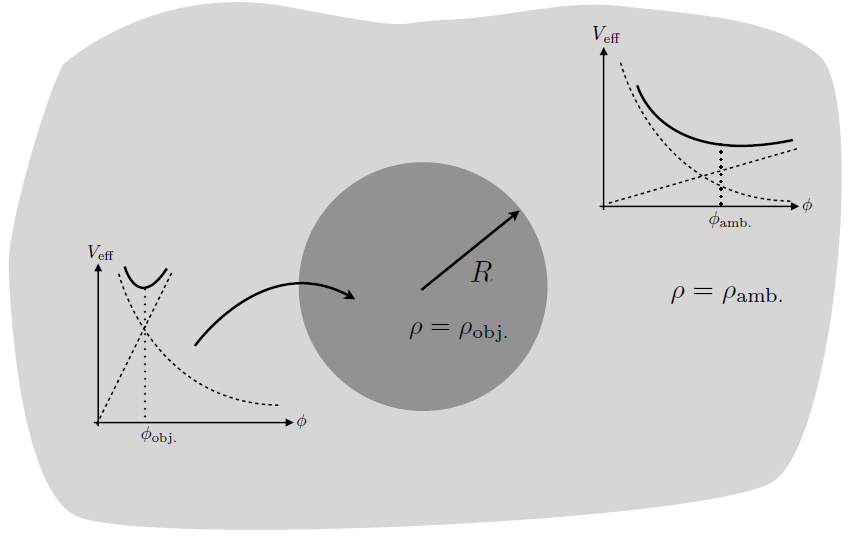
\includegraphics[scale=0.70]{modif_grav/eff_pot.png}
	\caption{The effective chameleon potential for a massive spherical object of density $\rho_{\mbox{\scriptsize{obj.}}}$ surrounded by the background with density $\rho_{\mbox{\scriptsize{amb.}}}$. From \textcite{2015PhR...568....1J}.}
	\label{fig_eff_pot}
\end{figure}

In spherical coordinates assuming spherical symmetry, equation \eqref{eq:cham} becomes
\eq{
\label{eq_cham_r}
\frac{\dd^2\phi}{\dd r^2}+\frac{2}{r}\dddd{\phi}{r}=\frac{1}{r}\frac{\dd^2\left(r\phi\right)}{\dd r^2}=V_{,\phi}\left(\phi(r)\right)+\frac{\beta}{\Mpl}\rho(r).
}
We must impose two boundary conditions which are
\begin{align*}
\dddd{\phi}{r}(r=0)&=0 \\
\phi(r\rightarrow\infty)&=\phi_\infty.
\end{align*}
The first one corresponds to a non-singularity of the solution at the origin while the later one ensures that the chameleon force vanishes at the infinity (as $\dd\phi/\dd r\rightarrow0$).

The equation \eqref{eq_cham_r} drives the field $\phi$ toward the $\phi_\infty$ outside the object and toward $\phi_c$ inside the object. Note that the second term acts like the friction term.

In order to solve \eqref{eq_cham_r} we must do several approximations. Outside the object we assume that the field sits near the extreme $\phi_\infty$ and we can linearized our equation
\eq{
\frac{1}{r}\frac{\dd^2\left(r\phi\right)}{\dd r^2}=m^2_\infty(\phi-\phi_\infty),
}
with the decaying solution
\eq{
\phi(r)=-\frac{\beta}{4\pi\Mpl}\frac{\tilde{M}}{r}e^{-m_\infty r}+\phi_\infty.
}
Note that the integration constant $\tilde{M}$ is not generally the mass of the object $M_c$ as in the case of the Newtonian potential because it is determined by the field inside the object which has different behavior than the Newtonian potential. As we will see later, for small Newtonian potentials (in magnitude) this effective mass $\tilde{M}\approx M_c$ but as the potential grows larger part of the object`s mass is screened away $\tilde{M}< M_c$.

Inside the object we use one of the two approximations based on the initial value of $\phi_i\equiv\phi(0)$ -- either $\phi_i\approx\phi_c$ or $\phi_i\gg\phi_c$ .
\subsubsection{Thin-shell regime}
In the \textit{thin-shell} regime the field initially sits very close the minimum $\phi_c$, i.e. we require
\eq{
(\phi_i-\phi_c)/\phi_c\ll1.
}
The field is frozen near this value until the friction term is sufficiently small to allow the field to roll. This ``moment'' is denoted by $R_{roll}$. As soon as $\phi$ is displaced significantly from $\phi_c$ we may neglect the potential term in \eqref{eq_cham_r}. This gives us the solution
\eq{
\phi(r)=
\begin{cases}
\phi_c & 0<r<R_{roll} \\
\frac{\beta}{6\Mpl}\rho_cr^2+\frac{A}{r}+D & R_{roll}<r<R_c.
\end{cases}
}
We have boundary conditions coming from the requirement on matching $\phi$ and  $\dd\phi/\dd r$ at $R_{roll}$, namely: $\phi=\phi_c$ and $\dd\phi/\dd r=0$ at $r=r_{roll}$. This fixes our constants and the solution is
\eq{
\label{eq_thin}
\phi(r)=
\begin{cases}
\phi_c & 0<r<R_{roll} \\
\frac{\beta\rho_c}{3\Mpl}\left(\frac{r^2}{2}+\frac{R^3_{roll}}{r}\right)-\frac{\beta\rho_cR^2_{roll}}{2\Mpl}+\phi_c & R_{roll}<r<R_c.
\end{cases}
}
The approximation of separating the solution into the two regions only makes sense if $(R_c-R_{roll})/R_c\ll1$. Otherwise there is no clear separation between the two regions, and one needs a solution valid over the entire range $0<r<R_c$. In \autoref{num_cham} is \eqref{eq_cham_r} solved numerically and we can check these approximations against numerical solutions.

With approximation $(R_c-R_{roll})/R_c\ll1$ we can determines the effective mass of the object $\tilde{M}$ from the requirement $\phi(R_c^-)=\phi(R_c^+)$ and $\dd\phi/\dd r(R_c^-)=\dd\phi/\dd r(R_c^+)$.
\eq{
\tilde{M}=\frac{3\Delta R_c}{R_c}M_c,
}
where
\eq{
\frac{\Delta R_c}{R_c}\equiv\frac{\phi_\infty-\phi_c}{6\beta\Mpl|\Phi_N(R_c)|}\approx\frac{R_c-R_{roll}}{R_c}\ll1.
}
This qualitative derivation of the thin-shell regime is using too much strong assumptions and can be done more precisely without ignoring some of the terms but then it is harder to see the principle of the thin-shell effect. For more details see e.g. \textcite{Tamaki:2008mf}, \textcite{2007PhRvD..75f3501M}, \textcite{Waterhouse:2006wv}.
\subsubsection{Thick-shell regime}
In the \textit{thick-shell} regime the field is initially sufficiently displaced from the minimum -- $\phi_i\gg\phi_c$ that it begins to roll almost immediately (no friction term). Hence the interior solution is most easily obtained by taking the $R_{roll}=0$ in \eqref{eq_thin} and replacing $\phi_c$ by $\phi_i$
\eq{
\label{eq_thick}
\phi(r)=\frac{\beta\rho_cr^2}{6\Mpl}+\phi_i\ \ \ 0<r<R_c.
}
By matching the interior and exterior solutions, we obtain
\eq{
\begin{split}
\phi_i &=\phi_\infty-3\beta\Mpl\Phi_N(R_c)\\
\tilde{M} &=M_c,
\end{split}
}
which is the linear regime with no screening. From the definition of $\Delta R_c/R_c$ we also obtain
\eq{
\frac{\Delta R_c}{R_c}\equiv\frac{\phi_\infty-\phi_c}{6\beta\Mpl|\Phi_N(R_c)|}>1.
}
\subsubsection{Thin-shell suppression factor}
The chameleon force outside the object (where experiments take place) comparing to the Newtonian force is
\eq{
\begin{split}
\label{eq_cham_suppression}
\frac{F_{thick}}{F_N}&=2\beta^2 \\
\frac{F_{thin}}{F_N}&=2\beta^2\frac{3\Mpl\left(\phi_\infty-\phi_c\right)}{\beta\rho_cR^2_c},
\end{split}
}
where we ignore the term $m_\infty r\ll1$. Therefore for the coupling $\beta$ of order unity the chameleon force is as strong as gravity unless it is screened away by the thin-shell effect.
%%%%%%%%%%%%%%%%%%%%%%%%%%%%%%
% HU-SAWICKI
%%%%%%%%%%%%%%%%%%%%%%%%%%%%%%
\subsection{Hu-Sawicki \texorpdfstring{\textit{\lowercase{f}(R)}}{fR} Model}
\todo{Cite own paper}
We wish to study a class of $f(R)$ models that accelerate cosmic expansion at late times, without the cosmological constant, while satisfying both cosmological and Solar System tests. We consider the family of Hu-Sawicki $f(R)$ models \parencite{Hu-Saw}. The action of these models is given by \eqref{eq:S_fr} and $f(R)$ has a broken power-law form
\eq{
	f(R)=-M^2\frac{c_1(R/M^2)^m}{c_2(R/M^2)^m+1}\,,
}
where the mass scale $M^2\equiv\bar\rho_0/3\Mpl^2$, $m>0$, and $c_1$ and $c_2$ are dimensionless parameters such that at high redshifts \LCDM\ cosmology is restored.

The formulation of modified gravity in this frame leads to second-order differential equations of motion \eqref{eq:fR} for $R$ and fourth-order field equations for $g_\uv$. With a conformal transformation we may rewrite these equation in the Einstein frame with second-order differentials only \parencite[see, e.g.,][]{CHIBA20031}.

In the Einstein frame \todo{see transformation eqref}, the Hu-Sawicki models correspond to chameleon gravity with the potential
\eq{
	V(\chi) &= \Mpl^2\Lambda-\frac{\beta\bar\rho_0}{n\Mpl}\left(2\beta\Mpl\Phiscrz\right)^{1-n}\chi^n\,, \\
    V_{,\chi}(\chi) &= -\frac{\beta}{\Mpl}\bar\rho_0\left(\frac{2\beta\Mpl\Phiscrz}{\chi}\right)^{1-n}\,,
}
where $\beta=\sqrt{1/6}$ and the power-law exponent $n$ and screening potential $\Phiscrz$ are parameters of the theory. The screening potential has the following relation to the present scalaron value in $f(R)$-gravity:
\todo{add eqref}
\eq{
    \Phiscrz=\frac{3}{2}\ln{(1+f_{R0})}\approx\frac{3}{2}f_{R0}.
}
The extra scalar degree of freedom $\chi$ (\textit{chameleon}) obeys the equation of motion
\eq{
	\Box \chi = V_{,\chi}(\chi) + \frac{\beta}{\Mpl}\rho\equiv V_{\eff,\chi}(\chi)\,.
}
When matter moves non-relativistically and we are inside the sound horizon of the chameleon, time derivatives may be neglected, hence
\eq{
\label{eq:cham}
	\Delta \chi = \frac{\beta}{\Mpl}\rho - \frac{\beta}{\Mpl}\bar\rho_0\left(\frac{2\beta\Mpl\Phiscrz}{\chi}\right)^{1-n}
}
The transformation from the Jordan frame to the Einstein frame introduces non-standard coupling of the chameleon field to standard matter. This results in a fifth force, given in the non-relativistic limit by
\eq{
    \label{eq:cham_force}
	\dddd{\mb u_{\chi}}{a} = -\frac{3\mu}{2a}\frac{\beta}{\Mpl}\vec{\nabla}\chi \,.
}
%%%%%%%%%%%%%%%%%%%%%%%%%%%%
% Other theries
%%%%%%%%%%%%%%%%%%%%%%%%%%%%
\section{Other theries}
In this section we briefly mention some of other theories od modified gravity. This list is in no way complete and serves only as an example of different approaches to modifications of gravity. See references for further reading.
\subsection{Quintessence}
Quintessence, from the Latin ``fifth element'', is according to ancient and medieval philosophy the fifth element, or ether, supposed to be the constituent matter of the heavenly bodies after air, fire, earth, and water. The name quintessence, or the $Q$ component, was first used by \textcite{1998PhRvL..80.1582C} for canonical scalar field $\phi$ evolving along a potential $V(\phi)$. Such a dynamical field can reproduce the late-time acceleration with the equation of state $w=w(t)\approx1$. Although quintessence can alleviate the coincidence problem of dark energy via the so-called tracker solution, it still suffers by the fine-tunning problem as the potential needs to be flat enough to lead to the slow-roll inflation today with an energy scale $\rho_{DE}\simeq10^{-120}\Mpl^4$ and a mass scale $m_\phi\lesssim10^{-33}$ eV. However, such fine-tunned potentials can be constructed within the framework of particle physics.

Quintessence is one of the simple models of dark energy as it is a canonical scalar field that interacts with all the other components only through standard gravity. The lagrangian density for the quintessence field is
\eq{
\label{Qlagr}
\LL_\phi=-\frac12(\partial\phi)^2-V(\phi)
}
We can compute the stress-energy tensor as
\eq{
T^\phi_\uv\equiv\frac{-2}{\dg}\frac{\delta(\dg\LL_\phi)}{\delta g^\uv}=\partial_\mu\phi\partial_\nu\phi-g^\uv\left(\frac12(\partial\phi)^2+V(\phi)\right).
}
Now, the energy density and pressure is given by components of the stress-energy tensor. For FLRW background and $\phi$ only time-dependent we get
\eq{
\rho_\phi=-T^0_0=\frac{1}{2}\dot{\phi}^2+V(\phi)\ \ \ \ p_\phi=\frac{1}{3}T^i_i=\frac{1}{2}\dot{\phi}^2-V(\phi).
}
Equation of state for the quintessence is then
\eq{
\label{eosQ}
w\equiv\frac{p}{\rho}=\frac{\dot{\phi}^2-2V(\phi)}{\dot{\phi}^2+2V(\phi)}\,.
}
We require the condition $w<-1/3$ to realize the late-time cosmic acceleration, which translates into the condition  $\dot{\phi}^2<V(\phi)$, i.e. the potential needs to be shallow enough for the field to evolve slowly along the potential. For a slow-rolling field such as $\dot{\phi}\ll V(\phi)$ equation of state \eqref{eosQ} reduce to $w\approx-1$ as indicated by cosmological measurements.

The variation of \eqref{Qlagr} with respect to $\phi$ gives us the equation of motion for the scalar field $\phi$
\eq{
\ddot{\phi}+3H\dot{\phi}^2+V_{,\phi}=0\,.
}

Depending on which term and when determines the evolution of the field, the quintessence models has been dynamically classified into \textit{freezing} models and \textit{thawing} models \parencite{2005PhRvL..95n1301C}. In the freezing models the field was rolling along the potential in the past, but the movement gradually slows down as the field approaches the minimum of the potential $(\dot{\phi}\rightarrow0)$ and the system enters the phase of the cosmic acceleration $(w\rightarrow-1)$. In the thawing models the field was initially frozen $(\dot{\phi}\approx0)$ in the early matter era because of the Hubble friction (the term $H\dot{\phi}$) until recently and then it begins to evolve once $H$ drops below $m_\phi$ and $w$ evolves from $-1$.

A potential of the freezing models is for example
\eq{
\label{Qtr}
V(\phi)=M^{4+n}\phi^{-n}\ (n>0),
}
which appears in the fermion condensate model as a dynamical supersymmetry breaking \parencite{1999PhRvD..60f3502B}. This potential does not possess a minimum and hence the field rolls down the potential toward infinity. Another example of a potential in the freezing models is
\eq{
V(\phi)=M^{4+n}\phi^{-n}\exp{(\alpha\phi^2/\Mpl^2)},
}
which can be constructed in the framework of supergravity \parencite{1999PhLB..468...40B}. This potential has a minimum at which the field is eventually trapped (corresponding to $\dot{\phi}=0$ and hence $w=-1$).

Broader class of potentials belonging to the thawing models are so-called hilltop quintessence models \parencite{2008PhRvD..78l3525D}, in which the scalar field is rolling near a local \textbf{maximum} in the potential but it begins to roll down around the present. A particularly example that is well-described by this model is the pseudo-Nambu-Goldstone Boson (PNGB) model of \textcite{1995PhRvL..75.2077F}, for which the potential is given by
\eq{
V(\phi)=M^{4}\left[\cos{(\phi/f)}+1\right].
}
\subsection{K--essence}
Quintessence models are based on a scalar field with a canonical kinetic term and a slowly varying potential. However, in the context of particle physics there appear scalar fields with non-canonical kinetic terms. In \textcite{1999PhLB..458..209A} it is shown that a large class of scalar fields with non-canonical kinetic terms can, without the help of potential terms, drive an inflationary evolution starting from rather generic initial conditions. The Lagrangian density for the k-essence is
\eq{
\label{Klagr}
\LL_K=P(\phi, X),
}
where $X=-\frac12(\partial\phi)^2$ is the canonical kinetic energy and the function $P(\phi, X)$ must vanish for $X\rightarrow0$ (otherwise there would be some potential term). 

The energy-momentum tensor of the k-essence is given by
\eq{
T^K_\uv\equiv\frac{-2}{\dg}\frac{\delta(\dg\LL_K)}{\delta g^\uv}=P_{,X}\partial_\mu\phi\partial_\nu\phi+g^\uv P,
}
which is of the form of a perfect fluid, $T_\uv=(\rho+p)u_\mu u_\nu+g_\uv p$, with a four-velocity $u_\mu=\partial_\mu\phi/\sqrt{2X}$, pressure $p_K=P$ and energy density
\eq{
\rho_K=2XP_{,X}-P.
}
The equation of state of the k-essence is then
\eq{
w_K=\frac{p_K}{\rho_K}=\frac{P}{2XP_{,X}-P},
}
which is $w_K\approx-1$, as long as the condition $XP_{,X}\ll P$ is satisfied.

In the low-energy effective string theory appear higher-order derivative terms coming from $\alpha$ and loop corrections to the tree-level action \parencite{2003PhR...373....1G}. The k-essence action for these theories is for example
\eq{
P=K(\phi)X+L(\phi)X^2.
}
Phantom or ghost scalar fields with a negative kinetic energy $-X$ and $w\lesssim-1$ can also fit the current observations. These ghost fields generally suffer from a quantum instability problem unless higher-order terms in $X$ or $\phi$ are taken into account in the Lagrangian density \parencite{2010deto.book.....A}. The action of so-called dilatonic ghost condensate model is \parencite{2004JCAP...07..004P}
\eq{
P=-X+e^{\kappa\lambda\phi}X^2/M^4.
}
\subsection{Gauss-Bonnet Dark Energy Models}
In \fR\ gravity one adds general function of the Ricci scalar. But in principle one can add general functions of the Ricci and Riemann tensors as well, e.g. $f(R,R_\uv R^\uv,R_{\alpha\beta\gamma\delta}R^{\alpha\beta\gamma\delta},...)$ \parencite{2005PhRvD..71f3513C}. These Lagrangians are generally plagued by the existence of ghosts.  However, there exists a combination of Ricci and Riemann tensors that keeps the equations at second-order in the metric and does not necessarily give rise to instabilities -- so-called Gauss-Bonnet term $\GB$ coupled to a scalar field
\eq{
\GB\equiv R^2-4R_\uv R^\uv+R_{\alpha\beta\gamma\delta}R^{\alpha\beta\gamma\delta}.
}
The Gauss-Bonnet term is the unique invariant for which the highest (second) derivative occurs linearly in the equations of motion and thus ensuring the uniqueness of solutions. The Gauss-Bonnet term naturally arises as a correction to the tree-level action of low-energy effective string theories \parencite{2000PhR...337..343L}. The starting action is given by
\eq{
S=\int\dd^4x\dg\left[\frac{\Mpl^2}{2}R-\frac{\gamma}{2}\left(\nabla\phi\right)^2-V(\phi)+f(\phi)\GB\right],
}
where $\gamma=\pm1$ (+1 for the canonical scalar). For more details see \textcite{2005PhRvD..71l3509N,2006JCAP...06..004N,2013PhRvD..87h4037C}.
\subsection{Braneworld Models}
In the braneworld model of Dvali, Gabadadze and Porrati \parencite[DGP model][]{2000PhLB..485..208D} the 3-brane is embedded in a Minkowski bulk spacetime with infinitely large extra dimensions. The theory gives rise to the correct 4D potential at short distances whereas at large distances the potential is that of a 5D theory. The action of the theory is
\eq{
S=\frac{M^3_{(5)}}{2}\int\dd^5X\dgt\tR+\frac{\Mpl^2}{2}\int\dd^4x\dg R + \int\dd^4x\dg \LL_m,
}
where $g_{AB}(X)=g_{AB}(x,y)$ denotes a 5D metric for which the 5D Ricci scalar is $\tR$ and $M_{(5)}$ is the 5D Planck mass. Capital letters are used for 5D quantities $(A,B=0,1,2,3,5)$. The brane is located at $y=0$. The induces 4D metric on the brane is denoted by
\eq{
g_\uv(x)\equiv\tilde{g}_\uv(x,y=0).
}
The cross-over scale $r_0$ is defined by
\eq{
r_0\equiv\frac{\Mpl^2}{2M^3_{(5)}}.
}
At short distances $r\ll r_0$ gravity behaves as usual 4D theory, i.e the gravitational potential has correct $1/r$ behavior (except small logarithmic repulsion term). On the other hand at large distances $r\gg r_0$ the potential scales as $1/r^2$ in accordance with laws of 5D theory.

The presence of the extra dimension has severe consequences on the cosmology as well. It can be shown \parencite{2010deto.book.....A,2009PhLB..674..237M} that the matter dominated Universe approaches the de Sitter solution $H=r_0\mins$. This cosmological solution drives our Universe into the self-inflationary regime without dark energy. From $H_0\approx r_0\mins$ we get $M_{(5)}\approx10-100$ MeV.
\subsection{Massive Gravity}
The idea to give a mass to the graviton (infrared modification of gravity) is not new and has been investigated since the first years of General Relativity. It is a less minimal theory than \fR\ theories or modified gravities with an extra scalar field because it introduces three new degrees of freedom rather than one. By giving a mass $m$ to the graviton we deform the classical potential to the Yukawa profile $\sim\frac1r e^{-mr}$ which departs from the classical one at distances $r>1/m$. By choosing the graviton mass to be of the order of the Hubble constant $m\sim H$ one can hope to explain the acceleration of the universe without dark energy.

The simplest theory for a non-self-interacting massive graviton is Fierz-Pauli theory of \textcite{1939RSPSA.173..211F}. The action for a single massive spin 2 particle in flat space, carried by a symmetric tensor field $h_\uv$ is
\eq{
\begin{split}
S=&\int\dd^4x\Big[-\frac12\partial_\lambda h_\uv\partial^\lambda h^\uv+\partial_\mu h_{\nu\lambda}\partial^\nu h^{\mu\lambda}-\partial_\mu h^\uv\partial_\nu h \\
&+\frac12\partial_\lambda h \partial^\lambda h-\frac12 m^2\left(h_\uv h^\uv-h^2\right)\Big]+S_m.
\end{split}
}
Any other combination of $h_\uv h^\uv$ and $h^2$ would lead to instabilities. Varying the action with respect to $h_\uv$ yields the equation of motion
\eq{
R_\uv-\frac12Rg_\uv+\frac12m^2(h_\uv-h\eta_\uv)=\frac{1}{\Mpl^2}T_\uv,
}
where all quantities are linearized around $\eta_\uv$.

Because of the so-called vDVZ discontinuity (``van Dam-Veltman-Zakharov'') in the propagator of a graviton, the Fierz-Pauli theory leads to different physical predictions from those of GR regardless the mass of the graviton (even when $m\to0$). The Vainshtein mechanism \parencite{1972PhLB...39..393V} allows in principle to get rid of the vDVZ discontinuity by introducing non-linear Fierz-Pauli gravity.

The Vainshtein mechanism is another example of the screening mechanism and restores the continuity with GR on scales below the so-called Vainshtein radius $r_V$, defined as
\eq{
r_V\equiv(GM/m^4)^{1/5}.
}
Much below the Vainshtein radius, which grows as the graviton`s mass approaches $0$, only linear terms plays crucial role and the GR is restored.

For more about the massive gravity and the Vainshtein mechanism see e.g. \textcite{2013CQGra..30r4001B,2012RvMP...84..671H}.

\subsection{Acceleration without Dark Energy}
So far we studied some kind of a dark energy -- either in a form of an exotic matter or by modifying gravity itself. But this need for a dark energy as an explanation of the acceleration comes from our observations which are based on the presumption of the homogeneous and isotropic Universe. What we observe are different expansion rates at different distances rather than an increase in the expansion rate at all distances. But this can be caused by strong inhomogeneities in the distribution of matter rather than by an accelerating Universe.
\subsubsection{Void models}
The basic idea behind void models is that we live in the middle of a huge spherical region which is expanding faster because it is emptier than the outside. That means that the Universe as a whole does not accelerate but that we observe an \textit{apparent} cosmic acceleration. The edge of this void should be located around $z\sim0.3-0.5$, the value at which in the standard interpretation we observe the beginning of the acceleration. These models are described by the Lema\^\i tre-Tolman-Bondi (LTB) spherically symmetric metric -- the generalization of a FLRW metric in which the expansion factor along the radial coordinate is different relative to the surface line element $\dd\Omega^2$ \parencite{2013JCAP...02..047D,2006PhRvD..73h3519A}.

The inhomogeneous LTB model matches to the supernovae data and the location of the first acoustic peak of CMB temperature power spectrum but cannot satisfactorily reproduce the entire CMB angular power spectrum \parencite{2011JCAP...02..013C}. The observed isotropy of the CMB radiation implies that we must live close to the center of the void -- nearer than 15 Mpc \parencite{2006PhRvD..74j3520A}. Moreover, there is no valid mechanism at present to explain the formation of such huge inhomogeneities, let alone one with our Galaxy near the center.
\subsubsection{Backreaction}
Unlike the void models, which regard the acceleration as an apparent one, \textit{backreaction} models try to explain the cosmic acceleration by arranging inhomogeneities so that the deviation from the FLRW metric can produce a real acceleration \parencite{2011CQGra..28w5002S,2004JCAP...02..003R,2005PhRvD..72b3507M}. Because GR equations are non-linear, averaging the inhomogeneities and then solving the GR equations (which is the usual approach) is not the same as first solving the full (inhomogeneous) GR equations and then averaging them -- the expected value of a non-linear function is not the same as the nonlinear function of the expected value.

Any large inhomogeneities must be conceal from our sight to fit observations. Strong peculiar velocities instead of strong density fluctuations can do this job, but there are strong constraints on peculiar velocities from e.g., the kinematic Sunyaev--Zel'dovich effect. Moreover, the accompanying anisotropy is another source of observable effects difficult to accommodate with current observations.